\chapter{Calidad de la Informaci\'on}

La \emph{calidad} tomada como su forma m\'as general, se define como la propiedad o conjunto de propiedades inherentes a algo, que permiten juzgar su valor. De manera m\'as particular, la informaci\'on que pretendemos que se encuentre en los documentos, debe cumplir con ciertos atributos que denotan la calidad de los documentos.

La determinaci\'on de las caracter\'isticas de calidad que ellos deben poseer puede variar dependiendo de los objetivos y el recurso tratado, sin embargo, algunas de ellas son comunes a todos los documentos como lo son:  contenido apropiado, actualizaci\'on, exactitud y accesibilidad entre otros.

La aparici\'on de algunas o todas las caracter\'isticas en los documentos trae aparejado un conjunto de ventajas tales como la mejora y precisi\'on del contenido.

\emph{Organizaci\'on del cap\'itulo.} La subsecci\'on 2.1 presenta una introducci\'on general al concepto de calidad. La subsecci\'on 2.2 se enfoca en mostrar aspectos de calidad relacionados a la Web. En la subsecci\'on 2.3 se introducen conceptos y caracter\'isticas que son considerados de calidad en los art\'iculos de Wikipedia. Al mismo tiempo se presentan los diferentes niveles de calidad existentes en dichos art\'iculos.

\section{Calidad de la informaci\'on general}

\section{Calidad de la informaci\'on en la Web}

Que \emph{``la informaci\'on es poder''}, se sabe desde hace mucho tiempo. Hoy en d\'ia, las demandas de informaci\'on aumentaron pasando a ser un bien necesario en nuestra vida diaria que debe ser actualizado constantemente para no quedar desfazado en el tiempo.
La informaci\'on puede ser definida como el mensaje usado para representar un hecho con el fin de incrementar el conocimiento y el aprendizaje, los cuales son cada vez m\'as necesarios para desarrollar cualquier actividad.

Cuando se hace uso de Internet para recoger informaci\'on, es necesario definir exactamente lo que se busca, que tipo de informaci\'on se necesita, cual es el objetivo de la b\'usqueda  y decidir fundamentalmente que fuentes son las m\'as confiables para poder satisfacerla, sobre todo teniendo en cuenta la gran variedad de material que se puede encontrar en la Web.

Cada d\'ia, surge nueva informaci\'on que es f\'acil y gratuitamente publicada en la Web, la cual se ha convertido en un potente medio de comunicaci\'on y difusi\'on en el que cualquier persona, organismo o empresa que disponga de una computadora y una conexi\'on a Internet, puede generar informaci\'on en la misma. Sumado a esto, se eliminan todas las barreras tradicionales de los medios de edici\'on impresa, donde para poder publicar se requiere pasar por un proceso de evaluaci\'on, de filtrado y de revisi\'on, y cumplir con las normas de publicaci\'on propias de cada editorial.

Debido a la propia naturaleza de la red, din\'amica, a menudo desorganizada y con informaci\'on dudosa o desconocida, la calidad de la informaci\'on ha sido desde sus or\'igenes cuestionada. En contraposici\'on, nos encontramos con la importancia que en el \'ambito de las Ciencias de la Documentaci\'on y de la Informaci\'on ha tenido siempre la evaluaci\'on tanto de la calidad de la informaci\'on como de los sistemas de recuperaci\'on de informaci\'on, con el objetivo de proporcionar al usuario la informaci\'on que necesita y que adem\'as sea \'util y de calidad. Como consecuencia directa, detectamos que los usuarios se enfrentan a unos nuevos retos como son localizar informaci\'on de calidad y \'util en la red, y evaluar dicha informaci\'on para verificar su calidad.

Queda en claro que la calidad de la informaci\'on actualmente es un concepto multidimensional que combina diversos factores ~\cite{WanStr:96}.
Una interpretaci\'on ampliamente aceptada de la calidad de la informaci\'on es la  ``aptitud para el uso en una aplicaci\'on pr\'actica''  ~\cite{WanStr:96}. De manera similar, Juran y Godfrey ~\cite{JurGod:99} interpretan la informaci\'on como ''de calidad si son aptas para los usos previstos en la operaci\'on'', es decir, dependiendo directamente del contexto en el que se aplica.

Otra definici\'on utilizada es la que sostiene que la calidad de la informaci\'on de un recurso ser\'a determinado por la capacidad de satisfacer las necesidades de informaci\'on de la persona que lo utilice o consulte, sin embargo, esto puede ser muy relativo, ya que la apreciaci\'on de la calidad es muy subjetiva, siendo para algunas personas de calidad lo que para otras no lo es. Lo que si podemos afirmar es que la calidad de la informaci\'on no es una realidad  medible de forma exacta y un\'ivoca sino que puede percibirse de diferentes dimensiones, y la cantidad de dimensiones que se tomen en cuenta determinar\'a la exhaustividad de su estudio.

En un principio, la diferencia entre calidad de datos e informaci\'on de calidad defin\'ia a la primera como ``la aptitud para el uso'', es decir, la capacidad de una colecci\'on de datos para satisfacer requisitos del usuario  ~\cite{StroD:97, CappC:02}. Por otro lado, calidad de datos es un concepto multidimensional ~\cite{CappC:02}. En la literatura se han atribuido categor\'ias y dimensiones para encarar problemas relacionados con la calidad de datos e informaci\'on de calidad. El marco mas utilizado es el propuesto por ~\cite{StroD:97}, el cual plantea una clasificaci\'on basada en la perspectiva del usuario como se muestra en el cuadro \ref{table:tablacidc1}.

\begin{table}[h]
  \centering
   \renewcommand{\arraystretch}{2}
   \begin{tabular}{>{\arraybackslash}m{3cm} >{\arraybackslash}m{10cm}}
	   \hline
	   \textbf{Categor\'ias} & \textbf{Dimensiones} \\
	   \hline
	   Intr\'inseca & Exactitud, Objetividad, Credibilidad, Reputaci\'on \\
	   Accesibilidad & Accesibilidad y Seguridad  \\
	   Contextual &  Relevancia, Valor a\~nadido, Oportunidad, Completitud, Informaci\'on Cantidad \\
	   Interpretabilidad representacional & F\'acil entendimiento, Representaci\'on concisa, Representaci\'on coherente  \\
\hline
 \end{tabular}
\caption {Categor\'ias y dimensiones para la calidad de la informaci\'on y datos de calidad.}
\label{table:tablacidc1}
\end{table}

Actualmente, no existe todav\'ia un consenso acerca de la distinci\'on entre datos de calidad e informaci\'on de calidad. Madnick ~\cite{MadWanLeeZhu:09}, determina el uso de calidad de datos refiri\'endose a detalles t\'ecnicos como la integraci\'on de registros de diferentes bases de datos, mientras que utiliza calidad de informaci\'on para referirse a detalles no t\'ecnicos como la importancia de la informaci\'on para cierto usuario, adem\'as de ofrecer una visi\'on global de las dimensiones de la calidad, incluyendo precisi\'on, confiabilidad, etc. Por otra parte, los te\'oricos de la informaci\'on, utilizan el t\'ermino \emph{dato} para referirse a textos planos que necesitan ser procesados para convertirse en informaci\'on \'util, mientras que \emph{calidad de la informaci\'on} es utilizado para referirse al resto de los casos. En un principio, las investigaciones acerca de informaci\'on de calidad y datos de calidad surgi\'o en los sistemas de informaci\'on ~\cite{StroD:97, LeeY:02}. Luego se extendi\'o a diferentes contextos, tales como sistemas cooperativos ~\cite{FugM:02, MarC:02}, almacenes de datos ~\cite{Bouze:01, ZhuBu:02} y comercio electr\'onico ~\cite{KatSia:99} entre otros.

La calidad de la informacion en Internet particularmente, requiere de un proceso continuo de planificaci\'on, an\'alisis, dise\~no, implementaci\'on, promoci\'on e innovaci\'on, con el fin de asegurar que se cubran las necesidades de los usuarios en cuanto a contenido, presentaci\'on y usabilidad. Sin embargo, debido al esfuerzo que requiere esta tarea sumado a la naturaleza ca\'otica de Internet, que dificulta la b\'usqueda, identificaci\'on y localizaci\'on de la informaci\'on deseada, muchas veces se deja de lado y hace que encontremos en Internet recursos de diferentes calidades. Pero el beneficio a largo plazo es mayor en t\'erminos de prestigio, marketing, difusi\'on del conocimiento, aunque es bien conocido por las personas o entidades que apuesten por la calidad de la informaci\'on que \'esta tiene un precio, un costo en t\'erminos econ\'omicos (tiempo que se tarda en publicar es mayor, las revisiones y mejoras requieren tiempo y personal).
Estas razones nos llevan a que si queremos ofrecer informaci\'on de calidad tengamos en cuenta que es un proceso de mejora constante, que implica llevar a cabo varias acciones, como por ejemplo:

\begin{itemize}
\item Uso de checklists o listas para la evaluaci\'on de la informaci\'on.
\item Hacer uso de la opini\'on de los usuarios acerca de la informaci\'on proporcionada.
\item Supervisi\'on y control de la informaci\'on que se publica.
\item Controles de calidad exhaustivos antes de la publicaci\'on.
\end{itemize}

Los documentos electr\'onicos, constan de dos componentes la forma y la informaci\'on. A pesar de que ambos son muy importantes, los usuarios, en general, se interesan m\'as en el contenido que en la forma en que se presenta el documento. Sirve de poco que la informaci\'on este completa y mal organizada y viceverza ~\cite{MaPiMo:11}.

El boom de la Internet trajo aparejado una creciente diversidad de contenidos dejando en evidencia que la evaluaci\'on de los documentos Web generados son un punto m\'as que importante. Esto permiti\'o la introducci\'on de m\'etricas  de calidad en los diferentes enfoques de recuperaci\'on de la informaci\'on como ranking sesgado, distancia de la colecci\'on de los documentos y radio de ruido de la informaci\'on, entre otros ~\cite{BenCroDia:11, PirTal:10, ZhoCro:05, ZhuGau:00}. Cabe destacar que no existe un indicador perfecto que nos mida la calidad o el valor de la informaci\'on. Algunos de ellos son mas f\'aciles de medir que otros ya que se encuentran muy relacionados entre si. ~\cite{Harrr:97} sostiene que determinar la calidad de la informaci\'on es un arte, ya que hay que inferir a partir de un conjunto de indicadores, basados en la utilidad o prop\'osito con el que se quiera utilizar la fuente de informaci\'on. De manera general, actualmente, pocas fuentes de informaci\'on van a satisfacer todos los criterios, sin embargo, la aplicaci\'on de los mismos es de gran utilidad para distinguir la informaci\'on de alta a la de baja calidad.

En el mundo de los negocios, por otro lado, el avance tecnol\'ogico y de Internet ha tenido un gran impacto  permitiendo la aparici\'on de diversas aplicaciones Web generando mayor competitividad, la cual, debe ser asegurada a trav\'es de la calidad de los datos en las aplicaciones utilizadas ~\cite{MaCcIcMp:05}.

A trav\'es del estudio de diferentes trabajos orientados a caracter\'isticas de calidad en los documentos Web, podemos rescatar la siguiente informaci\'on: precisi\'on, completitud y puntualidad, las cuales se fijan como las m\'as estudiadas, destac\'andose en la mayor\'ia de los trabajos. En menor medida encontramos las caracter\'isticas consistente, conciso, actualizado, interpretabilidad, relevancia, seguridad, accesibilidad, cantidad apropiada de datos, disponibilidad, credibilidad, objetividad, reputaci\'on, fiabilidad de la fuente y trazabilidad (rastreable). En menor medida, detectamos como caracter\'isticas de calidad en los documentos Web la confidencialidad, la conveniencia, el grado de duplicados y de granularidad y la flexibilidad entre otros. Cabe destacar que varias de las caracter\'isticas nombradas anteriormente se incluyen en las normas internacionales de calidad de software, sin embargo, no todas se consideran en el mismo nivel en este tipo de normas, por ejemplo disponibilidad y comprensibilidad. En resumen, hay una serie de convenciones universalmente aceptadas de las caracter\'isticas deseables de la informaci\'on, entre las cuales encontramos la \emph{objetividad} en primer lugar, la \emph{integridad} y la \emph{utilidad}.

Por otro lado, y como aporte complementario, podemos considerar las valoraciones m\'as frecuentes de un sitio Web entre las cuales encontramos el \emph{mantenimiento y la actualizaci\'on}, especificando cuando fue revisado por \'ultima vez, si el contenido es est\'atico o din\'amico; \emph{si existen enlaces a otros sitios}, si estan \emph{actualizados}, si la informaci\'on presentada es \emph{simple y confiable}, si son de \emph{utilidad y  mostrados de forma clara y visible}, si son \emph{relevantes para el tema en cuesti\'on}; \emph{dise\~no y estructura de las p\'aginas del sitio}, refiri\'endose a como esta organizada y estructurada la informaci\'on, permitiendo un acceso f\'acil y l\'ogico; \emph{estabilidad}, haciendo alusi\'on a si a lo largo del tiempo se mantiene la URL, \emph{acceso al sitio}, facilidad de conexi\'on, descarga r\'apida, \emph{aporte gr\'afico}, si las im\'agenes o audios inclu\'idos en el sitio hacen un aporte importante y apropiado, si hace ameno el contenido presentado y por \'ultimo, \emph{requisito adicional de software o hardware}, haciendo hincapi\'e en que los sitios de calidad deber\'ian poder ser accesibles para cualquier usuario de Internet, independientemente de los programas o de la computadora utilizada.

Existen problemas que afectan directamente la calidad de la informaci\'on y los datos en la Web, como consecuencia de la naturaleza de la Web, como lo son informaci\'on desactualizada, problemas de dise\~no que hacen dif\'icil al usuario el acceso a la informaci\'on, publicaciones de informaci\'on inconsistente, v\'inculos obsoletos, etc ~\cite{EppMue:02}. En el campo del comercio electr\'onico, si los datos no son de calidad, es posible que la empresa tenga grandes p\'erdidas econ\'omicas y de imagen ~\cite{LimChi:00, HaiKor:03}.
Tambi\'en, el dinamismo en la Web ~\cite{Amir:03}, el uso e interacci\'on de diferentes fuentes externas, los servicios en tiempo real y en particular, los cambios que sufren las fuentes y datos constantemente ~\cite{PerbScam:02, Germ:04} pueden afectar directamente la calidad de la informaci\'on.

Otra de las situaciones t\'ipicas encontradas en la Web es la integraci\'on de datos estructurados con datos no estructurados ~\cite{FincAikp:99} adem\'as de la conexi\'on de datos diferentes ~\cite{ZhuBu:02, AngpMacl:04, BoumPerv:04, Germ:04}. En ambos casos, el desaf\'io mayor, se encuentra en conectar informaci\'on con diferentes niveles de calidad y entregarlo al usuario listo para su uso. Bajo este mismo contexto, es importante el enfoque desde la perspectiva desde los usuarios y la ayuda para entender los datos y su calidad, el uso de un lenguaje com\'un para facilitar la comunicaci\'on entre las personas, sistemas, etc ~\cite{AngpMacl:04, Cappc:04}.

Los m\'etodos de evaluaci\'on y mejora de la calidad de la informaci\'on en una aplicaci\'on Web son muy variados. Por ejemplo, en el trabajo de ~\cite{KatSia:99}, proponen un instrumento de evaluaci\'on para sitios Web individuales, a trav\'es de un formulario con 41 preguntas divididas en grupos, ~\cite{ZhuBu:02} establecen un conjunto de criterios para la evaluaci\'on y selecci\'on de recursos Web como fuente de datos externa, considerando tambi\'en, criterios de evaluaci\'on agrupados en tres categor\'ias (estabilidad de la fuente, calidad de datos y aplicaciones espec\'ificas). Estos m\'etodos son utilizados por organizaciones y managers de tecnolog\'ias de la informaci\'on para capturar el estado de la informaci\'on.

Queda claro que la Web debe adquirir mecanismos que hagan frente a estos cambios para lograr una evoluci\'on dr\'astica hacia la calidad de los datos utilizados en la misma. Surge al mismo tiempo, la necesidad de definir un marco general de calidad para los datos en la Web que incluyan todas las caracter\'isticas, inclusive aquellas con diferentes perspectivas del usuario.


Las dimensiones nombradas de la calidad de la informaci\'on pueden ser agrupadas en cuatro categor\'ias: intr\'inseca, contextual, representacional y accesibilidad. \\

\emph{La calidad intr\'inseca de la informaci\'on}, hace referencia al valor objetivo de la informaci\'on independientemente de su forma, difusi\'on, dise\~no o p\'ublico al que se lo dirige.
\begin{itemize}
\item \emph{Rigor cient\'ifico:} Es importante que dicha informaci\'on este respaldada por evidencia cient\'ifica, en m\'etodos cient\'ificos basados en cada una de las disciplinas.
\item \emph{Integridad:} la informaci\'on no debe ser parcial ni sesgada, presentada en su totalidad siempre y cuando no sea otro el objetivo (resumen).
\item \emph{Objetividad:} un aspecto que no es f\'acil de percibir, la credibilidad de la informaci\'on se asocia a la confianza que tenemos en el responsable del contenido en funci\'on de su autoridad. La carencia de esta caracter\'istica puede llevar a percepciones err\'oneas o desinformaci\'on. Cabe destacar que la objetividad depende del autor de la misma y no de la percepci\'on del usuario.
\item \emph{Precisi\'on:} este aspecto se relaciona con la exactitud de la informaci\'on y con la profundidad con las que se aborda un tema. Esta dimensi\'on depende de la intenci\'on y las pretensiones del recurso y a los usuarios a la que va dirigido.
\end{itemize}

\emph{La calidad contextual de la informaci\'on} hace alusi\'on al contexto en el que se accede a la informaci\'on y a la adecuaci\'on del usuario. Encontramos aqu\'i los siguientes aspectos:
\begin{itemize}
\item \emph{Relevancia:} implica cuanto se adecua la informaci\'on a las necesidades del usuario, dimensi\'on subjetiva ya que depende del tipo de usuario.
\item \emph{Valor a\~nadido:} estos elementos facilitan el uso de la informaci\'on para una mejor asimilacion de la misma, mejorando la calidad.
\item \emph{Actualidad de la informaci\'on:} exceptuando la informaci\'on con valor hist\'orico, esta carater\'istica determina calidad sobre todo en informaci\'on cient\'ifica o noticias.
\item \emph{Cantidad de informaci\'on aportada:} a mayor informaci\'on aportada, mejor ser\'a, siempre teniendo en cuenta los l\'imites del sistema en el que se cargan los datos.
\item \emph{Utilidad:} esta caracter\'istica tiene tanto un aspecto subjetivo, ya que mide cuan \'util es la informaci\'on y esto depende del tipo de usuario, mientras que por otro lado, la finalidad y el perfil del usuario al que se dirige aporta un aspecto objetivo.
\item \emph{Adecuaci\'on al usuario:} este aspecto depende puramente del usuario, pero es importante aclarar a qui\'en va dirigida la informaci\'on y adecuarla a ese perfil.
\end{itemize}

\emph{Calidad representacional de la informaci\'on}. Se relaciona con la forma en que se representa la informaci\'on, as\'i como tambi\'en todos los aspectos t\'ecnicos referidos a su estructura. En esta categor\'ia encontramos la claridad, concisi\'on, compatibilidad, dise\~no, flexibilidad, homogeneidad de los datos y tipos de formatos.

\emph{Calidad del acceso a la informaci\'on}. En esta categor\'ia se engloban los aspectos relativos al c\'omo se accede a la informaci\'on, como lo son \emph{tiempo de espera}, \emph{navegaci\'on} y \emph{seguridad} ~\cite{MaPiMo:11}.

Actualmente, resulta de vital importancia que dispongamos de criterios claros y funcionales para la evaluaci\'on y selecci\'on debido a la facilidad de publicar y la cantidad de documentos en la Web, para que el usuario  pueda discernir la veracidad, credibilidad, fiabilidad y la calidad de las informaciones de este medio. Esto puede verse claramente en entornos profesionales, como el acad\'emico y el cient\'ifico que requieren de recursos de informaci\'on mas rigurosos y pertinentes, o el mundo empresarial y comercial cuyos clientes exigen una informaci\'on veraz, organizada y de calidad ~\cite{MaPiMo:11}.

En el ambiente Web, aunque no todos persiguen los mismos objetivos y criterios, muchos son los profesionales que se dedican a evaluar los contenidos electr\'onicos. De forma general, se distinguen los grupos de profesionales, expertos, sociedades cient\'ificas, universidades, documentalistas y agencias de evaluaci\'on. Cada uno de estos grupos aporta un valor a\~nadido a los recursos electr\'onicos de portales y directorios.

Respecto a los criterios de evaluaci\'on, la calidad de la informaci\'on electr\'onica, puede ser evaluada desde diferentes perspectivas, aunque la m\'as com\'un es aquella que se centra en la satisfacci\'on del usuario. Debemos considerar que siempre antes de comenzar a analizar, se debe identificar la tipolog\'ia del documento ya que existe una gran variedad de gamas de recursos como lo son p\'aginas personales, Web comercial, etc. Los criterios e indicadores variar\'an en funci\'on de las caracter\'isticas de los recursos as\'i como tambi\'en del nivel de profundidad que desee emplear el evaluador.
La naturaleza hipertextual de la Web exige considerar dos niveles de evaluaci\'on sobre los que hay que aplicar criterios e indicadores:

\begin{itemize}
\item \emph{Micronavegaci\'on:} se refiere a todos los aspectos relacionados con la navegaci\'on interna entre los propios contenidos del sitio Web.

\item \emph{Macronavegaci\'on:} relacionada con los enlaces del sitio Web hacia el exterior y la visibilidad del mismo en todo el entorno de la Internet.
\end{itemize}

A continuaci\'on se presentan algunos criterios y par\'ametros aplicados a cada uno de estos niveles.

\begin{itemize}
\item \emph{Autor\'ia:} indispensable para distinguir la credibilidad de la fuente de informaci\'on. El responsable de los contenidos debe ser claramente identificado mediante algun indicador, como por ejemplo breve descripci\'on del curriculum del responsable, una adscripci\'on del autor a la organizaci\'on a la que pertenece, algun logotipo que represente a la instituci\'on, etc.
\item \emph{Actualizaci\'on:} se relaciona a la actualidad de los contenidos del sitio Web. Entre los indicadores m\'as comunes encontramos la indicaci\'on expl\'icita de la fecha de creaci\'on del sitio Web, la indicaci\'on expl\'icita de la fecha de actualizaci\'on de los contenidos, la correcta existencia de v\'inculos, etc.
\item \emph{Contenido:} Este criterio engloba varios requerimientos propios de los contenidos proporcionados en un sitio Web. Entre los m\'as destacados encontramos:
\begin{itemize}
\item \emph{Cobertura:} Este indicador valora el nivel de los contenidos tratados en el sitio Web.
\item \emph{Exactitud, precisi\'on y rigor:} la exactitud de los contenidos incluidos en un sitio Web deben poder ser verificables, como por ejemplo, desde el punto de vista cient\'ifico, apoyarse en citas bibliogr\'aficas, etc.
\item \emph{Pertinencia:} Se relaciona con la validez y utilidad de los contenidos incluidos en el sitio Web, valorando tanto los prop\'ositos declarados por el creador de los contenidos como el inter\'es que posea la informaci\'on para el usuario.
\item \emph{Objetividad:} se intenta identificar en la informaci\'on, presencia o ausencia de cualquier sesgo ideol\'ogico, pol\'itico o comercial.
\end{itemize}
\item \emph{Accesibilidad:} se refiere a todas las caracter\'isticas que hacen que el sitio Web sea accesible, sin dificultades para los diferentes usuarios. Entre lo m\'as destacado nos encontramos con: dise\~no compatible con diferentes navegadores o diferentes resoluciones de pantalla, existencia de versiones alternativas de visualizaci\'on para los sitios Web, posibilidad de imprimir, existencia de ayuda al usuario, etc.
\item \emph{Funcionalidad:} este criterio valora  la efectivdad del sitio Web a la hora de utilizarlo y consultarlo. Entre los indicadores b\'asicos que se deben tener en cuenta para valorar este criterio encontramos una estructura l\'ogica de los contenidos, pertinencia y adecuaci\'on de t\'itulos utilizados, la existencia de un mapa Web y de un sistema de b\'usqueda de contenidos propios del sitio Web.
\item \emph{Navegabilidad:} este criterio hace alusi\'on a la facilidad con que el usuario se puede desplazar en las p\'aginas de un sitio Web, aspecto relacionado con el conjunto de recursos y estrategias de navegaci\'on para conseguir un resultado \'optimo a la hora de encontrar la informaci\'on. Los indicadores que se rescatan de este criterio son presencia de un men\'u de contenidos siempre visible asi como tambien presencia de botones de navegaci\'on que permitan al usuario recorrer el sitio Web de manera l\'ogica.
\item \emph{Dise\~no:} aqu\'i se valora que el recurso, el documento Web, sea un espacio agradable a la vista y f\'acil de leer por el usuario
Dentro de este apartado se valoran varias cuestiones relacionadas con el aspecto f\'isico o la ergonom\'ia del sitio Web que contribuyen a hacer del recurso digital un espacio agradable a la vista y f\'acil de leer por el usuario. Los indicadores que aportar\'ian informaci\'on engloban un dise\~no Web elegante, funcional y atractivo, adecuada combinaci\'on de colores, formas e im\'agenes que faciliten la lectura de los contenidos, Tipograf\'ia adecuada, homogeneidad de estilo y formato en todas las p\'aginas del sitio Web. ~\cite{MaPiMo:11}
\end{itemize}

Como elemento final, en el cuadro \ref{table:problemas} detallamos los tipos de problemas de la calidad de la informaci\'on junto con sus posibles causas y acciones tomadas.

\section{Calidad de la informaci\'on en Wikipedia}

Gracias a su gran escala, continua evoluci\'on y de colaboraci\'on abierta, Wikipedia se ha convertido en un recurso muy popular en nuestros d\'ias proporcionando informaci\'on valiosa a los usuarios de Internet, adem\'as de plantear nuevos e importantes retos en diferentes \'areas de la organizaci\'on de la informaci\'on, incluyendo la calidad de la informaci\'on.

La definici\'on de calidad, como se mencion\'o anteriormente, depende del contexto, por lo que no existe ning\'un modelo fijo de garant\'ia de \emph{Informaci\'on de Calidad} que se pueda aplicar a todos los sistemas. En Wikipedia el contexto est\'a bien definido bajo el g\'enero enciclopedia. Sin embargo, la calidad de un art\'iculo enciclop\'edico definido en esta Web difiere actualmente al definido por Crawford ~\cite{Crawf:01} orientado a la enciclopedia escrita en papel, para la cual se determinan siete criterios generales: \'ambito, formato, unicidad, autoridad, exactitud, vigencia y accesibilidad. \\

La calidad de la informaci\'on en Wikipedia se formaliz\'o a trav\'es del \emph{art\'iculo destacado}. Estos son considerados como los mejores art\'iculos que Wikipedia puede ofrecer. \\

Dichos art\'iculos deben cumplir con\footnote{Art\'iculo destacado. https://en.wikipedia.org/?title=Wikipedia:Featured\_articles.
}:

\begin{enumerate}
	\item Estar bien escrito, completo, bien investigado, neutral y estable.
	\item Proporcionar una secci\'on concisa, una estructura apropiada y citas apropiadas.
	\item Contar con im\'agenes y otros medios visuales.
	\item Tener una longitud razonable y nivel de detalle.
\end{enumerate}

El Cuadro \ref{table:clas-calid}  muestra la clasificaci\'on de los diferentes niveles de calidad que puede tener un art\'iculo en Wikipedia\footnote{Niveles de calidad en un art\'iculo. \\ http://en.wikipedia.org/wiki/Wikipedia:Version\_1.0\_Editorial\_Team/Assessment. }.

\begin{table}
\begin{center}
\renewcommand{\arraystretch}{0.9}
\begin{tabular}{l  l  r}
	\hline
	& & \\
	{\bf Categor\'ia}	& {\bf Descripci\'on}									& {\bf Art\'iculos} \\ \\
	\hline
	& & \\
	FA 			& \emph{Featured Article, art\'iculo destacado}.  \\
				& Un art\'iculo marcado como la mayor obra de Wikipedia. \\
				& Distinguido por est\'andares profesionales de escritura, \\
				& presentaci\'on y fuentes.  & 4321 \\ \\
	A 			& \emph{A-Class, Clase A}.  \\
				& El art\'iculo est\'a bien organizado y completo, habiendo sido \\
				& revisado por evaluadores imparciales de WikiProject u otros. & 1054 \\ \\
	GA 			& \emph{Good Article, Buen Art\'iculo}.  \\
				& Un buen art\'iculo es un art\'iculo satisfactorio \\
				& que ha alcanzado los buenos criterios, pero no ha encontrado  \\
				& el criterio de art\'iculo destacado. & 16753 \\ \\
	B 			& \emph{B-Class, Clase B}.  \\
				& El art\'iculo est\'a completo en su mayor\'ia pero \\
				& requiere cierto trabajo futuro para alcanzar los est\'andares \\
				& de un buen art\'iculo. & 83523 \\ \\		
	C 			& \emph{C-Class, Clase C}.  \\
				& El art\'iculo es importante, pero a\'un contiene una gran  \\
				& cantidad de material irrelevante. El art\'iculo deber\'ia tener \\
				& referencias a fuentes fiables. Puede tener problemas \\
				& significativos o requerir limpieza sustancial. & 132444 \\ \\
	Start 			& \emph{Start, Inicio}.  \\
				& Un art\'iculo que est\'a desarrollado, pero que se encuentra \\
				& bastante incompleto y podr\'ia requerir fuentes confiables. & 904086 \\ \\
	Stub 			& \emph{Stub, Esqueleto}.  \\
				& Una descripci\'on muy b\'asica del tema. & 2206104 \\ \\
	FL 			& \emph{Featured List, Lista de caracter\'isticas}.  \\
				& Cubre un tema que conduce a la lista de formatos. \\
				& Son conocidas como las mejores listas en Wikipedia. & 1790 \\ \\					
	List 			& \emph{List, Lista}.  \\
				& Cumple con los criterios de una lista independiente,  \\
				& que es un art\'iculo que contiene principalmente una lista, \\
				& que por lo general consta de enlaces a art\'iculos \\
				& en un \'area tem\'atica particular. & 104209 \\ \\	
				&											& ---------- \\
				&											& 3454284 \\

	\hline
\end{tabular}
\end{center}
\caption{Esquema de clasificaci\'on de la calidad de los art\'iculos que componen la Wikipedia en Ingl\'es, junto con una descripci\'on de los criterios respectivos y el correspondiente n\'umero de art\'iculos que posee dicha categor\'ia.}
\label{table:clas-calid}
\end{table}

Los principales componentes del marco de aseguramiento de la calidad de Wikipedia son coordinaci\'on de trabajo y artefactos de soporte, roles y procesos. Este marco asume al menos 3 tipos de procesos:

\begin{itemize}
\item Los que evaluan la calidad de un art\'iculo y act\'uan directamente sobre este modific\'andolo, elimin\'andolo o cambiando su estatus.
\item Los que evaluan la performance de los editores de Wikipedia y seleccionan agentes que aseguran la calidad (administradores, bots, etc.).
\item Los que construyen y mantienen los artefactos de la coordinaci\'on de trabajo de Wikipedia.
\end{itemize}

Estos procesos nombrados pueden afectar la calidad de los art\'iculos de Wikipedia directa o indirectamente, modificando su contenido as\'i como tambi\'en el flujo de trabajo. Identifiquemos a continuaci\'on elementos existentes en Wikipedia que podr\'ian afectar la calidad de la informaci\'on en Wikipedia.

Con una comunidad ``hambrienta'' a contribuir, Wikipedia permite a los usuarios elegir en que art\'iculos y procesos contribuir y que roles tomar. Entre los roles detectados encontramos:

\begin{itemize}
\item \emph{Editores:} son aquellos agentes que contribuyen directamente en los art\'iculos.
\item \emph{Agentes de aseguramiento de la calidad:}  son agentes que afectan la calidad del art\'iculo, como lo son lo que revierten instancias de vandalismo, mejoras de la calidad del art\'iculo a traves de ediciones menores, etc.
\item \emph{Agentes maliciosos:} son aquellos que degradan la calidad de un art\'iculo a prop\'osito.
\item \emph{Agentes ambientales:} son aquellos que modifican la calidad de un art\'iculo por cambios producidos en el mundo real.
Aunque la mayor\'ia de las veces estos agentes degradan la calidad de los art\'iculos, en algunos casos pueden mejorarlos alineando el estado del mundo real con la informaci\'on contenida en un art\'iculo.
\end{itemize}

Por otra parte, se puede afirmar que Wikipedia no provee un sistema con usuarios con diferentes niveles de permisos, sin embargo, podemos encontrar tres grupos de cuentas:

\begin{itemize}
\item \emph{Usuarios registrados:} identificados por el nombre con el que ingresan a Wikipedia
\item \emph{Usuarios an\'onimos:} identificados por el protocolo IP.
\item \emph{Usuarios administradores y bur\'ocractas:} son usuarios registrados que poseen diferentes privilegios dentro de Wikipedia para editar los art\'iculos.
\end{itemize}

Tanto los usuarios an\'onimos como los usuarios registrados, pueden asumir diferentes roles en cualquier momento, por ejemplo, los usuarios registrados podr\'ian ser editores, agentes de calidad de la informaci\'on o agentes maliciosos. En el caso de los administradores, aunque es probable que degraden un art\'iculo, generalmente se espera que mejoren los art\'iculos, cumpliendo un rol de editores o agentes de la calidad de la informaci\'on.
Aunque como dijimos anteriormente, Wikipedia permite que los usuarios seleccionen ellos mismos los roles y procesos, tambi\'en promueve mecanismos para detectar buenos de malos editores y de esta forma moderar el trabajo sobre la informaci\'on. Aquellos editores que esten dispuestos a mejorar la calidad de la informaci\'on son promovidos a administradores dependiendo de su performance, conocimiento de Wikipedia, etc. Los administradores, poseen privilegios que les permiten, entre otras cosas, proteger, borrar, editar y restaurar art\'iculos. Por otro lado, los bur\'ocratas, son administradores como se indic\'o anteriormente, pero tienen todos los permisos de administradores, pudiendo realizar cualquier tarea dentro de Wikipedia.

Vale destacar que el modelo de aseguramiento de la calidad de Wikipedia tiene dos mecanismos para controlar y hacer cumplir la calidad de los art\'iculos:

\begin{itemize}
\item Asignaci\'on de un estatus ``Art\'iculo destacado", los cuales poseen un nivel alto deseado de calidad.
\item Procesos de eliminaci\'on del art\'iculo, que fuerzan a un m\'inimo nivel de calidad.
\end{itemize}

Es importante destacar que el n\'umero de art\'iculos destacados dentro de Wikipedia es muy peque\~no, rondando el 1\% del total de los art\'iculos de Wikipedia en Ingl\'es. Dichos art\'iculos destacados, son aquellos que corresponden a los mejores art\'iculos que Wikipedia puede ofrecer, seg\'un lo determinado por los Wikipedians, editores de Wikipedia. Los candidatos a art\'iculos destacados son revisados para determinar precisi\'on, neutralidad, integridad y estilo, de acuerdo a los criterios de los art\'iculos destacados.
Actualmente se cuenta con 4308 art\'iculos destacados de aproximadamente 4.500.000 en Ingl\'es. Esto nos indica que se posee 0.1\% de ellos, un valor muy bajo.
El art\'iculo destacado es representado en el sitio Web a trav\'es del icono de una estrella de bronce en la esquina superior derecha. Adem\'as, si el art\'iculo, tambi\'en es destacado en otros idiomas, una estrella aparecer\'a luego del v\'inculo del lenguaje en la lista posicionada del lado izquierdo de la p\'agina Web.

Los art\'iculos pueden ser nominados como candidatos a art\'iculo destacado por individuos o un grupo. Luego de nominados, los art\'iculos  candidatos son sometidos a una revisi\'on para comprobar si cumplen con los criterios de art\'iculos destacados. Seg\'un los registros de los art\'iculos destacados, el proceso se inici\'o en abril del 2002, aunque durante ese tiempo ning\'un art\'iculo se someti\'o a un proceso de revisi\'on por pares\footnote{Revisi\'on por pares. http://es.wikipedia.org/wiki/Revisi\'on\_por\_pares}, ni se hacia referencia a ning\'un criterio de evaluaci\'on, solo eran llamados art\'iculos con "buena prosa".

Una definici\'on mas general utilizada es ``aptitud para el uso'' ~\cite{JurJ:92}, mientras que una definici\'on mas operacional, incluye dimensiones de evaluaci\'on de calidad del contexto.

La primera gu\'ia para evaluar la calidad de la informaci\'on fue escrita por la elocuencia del usuario en el a\~no 2004. Esta gu\'ia inclu\'ia criterios como completitud, ajuste a los hechos y bien escrito. Esta gu\'ia fue sometida, luego, a m\'ultiples cambios, actualmente incluyendo 8 criterios de evaluaci\'on: completo, preciso y verificable con referencias, estable sin cambios frecuentes, bien escrito, no controversial con lenguaje neutro, cumplimiento de normas estandares de Wikipedia, tener im\'agenes correctas con su copyright y por \'ultimo, que tenga una longitud apropiada.

Aunque algunas de las dimensiones enumeradas en el modelo de Wikipedia como lo son estable, no controversial y verificable, no se enumeran en el marco de Crawford ~\cite{CrawH:01}, podemos deducir que se dan por sentadas.
La figura ~\ref{fig:jobInformationDialog} mapea las dimensiones de Crawford ~\cite{CrawH:01} con el modelo de Wikipedia nombrado y el marco posterior creado por Stvilia ~\cite{GasStv:01}.

\begin{figure}[h!]
	\begin{center}
		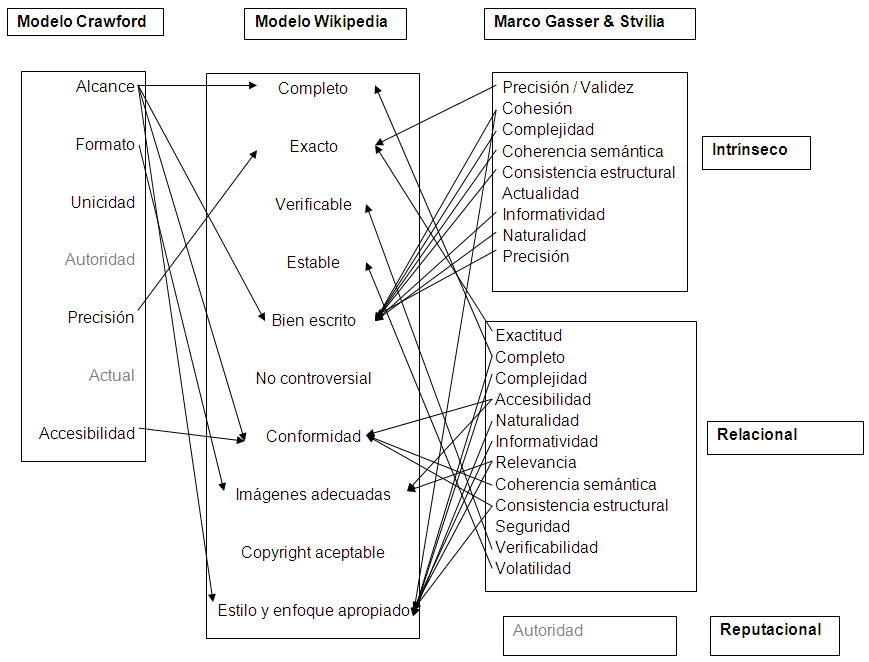
\includegraphics[width=1\textwidth]{imagenes/mapeo.png}
		\caption{Mapeo de las dimensiones de Crawford contra el modelo de Wikipedia y el marco creado por Stvilia}
		\label{fig:jobInformationDialog}
	\end{center}
\end{figure}

Por otro lado, en Wikipedia, tambi\'en se puede nominar un art\'iculo destacado para que sea removido de ese status. Entre los a\~nos 2004 / 2005,  aproximadamente 120 art\'iculos fueron nominados para ser removidos, y solo a 80 de ellos se les quit\'o la categor\'ia de art\'iculo destacado.

\begin{table}
  \centering
   \begin{tabular}{ l l l }
	\hline
	& & \\
	   \textbf{Problema} & \textbf{Causa} & \textbf{Acci\'on Tomada} \\ \\
	\hline
	& & \\
		Accesibilidad & Organizaci\'on Pobre. Pol\'iticas  & Reorganizar, duplicar,  \\
		& internas de Wikipedia. Barrera  & remover, traducir, unir. \\
		& del lenguaje. Copyright. & \\ \\
		Exactitud & Errores de tipeo. Cambios en el & Ajustar, corregir, cambiar,  \\
		&  mundo real. Bajo dominio del & actualizar, verificar, explicar,\\
		& idioma. Ilegible por software. & clarificar el contexto, remover. \\ \\
		Autoridad & Falta de fuentes de soporte. & Reformular, calificar, \\
		& Sesgo conocido de la fuente. & a\~nadir, sustituir, eliminar, \\
		& Generalizaci\'on infundada.  &   \\ \\
     	          Cohesi\'on & P\'erdida de foco. & Restringir, mover. \\ \\
     	          Completitud & M\'ultiples perspectivas. Falta de &  A\~nadir, especificar, \\
     	          & detalles. Cobertura desequilibrada  &  eliminar ambig\"{u}edad, incluir, \\
     	          & de diferentes perspectivas. &  equilibrar, calificar, aclarar, \\
     	          & & integrar, exponer. \\ \\
     	          Complejidad &  Baja Legibilidad. & Reemplazar, reescribir,  \\
		& Lenguaje complejo. & simplificar, mover, resumir.  \\ \\
     	          Consistencia & No cumplir normas sugeridas. & Reorganizar, voto,  \\
     	          & Diferencias en la sem\'antica del  & conformar, revertir, \\
     	          &  lenguage. Contradicci\'on de hechos, & elegir la forma mas usada. \\
     	          & cultura o norma social. & \\ \\
     	          Informatividad & Redundancia de contenido. & Remover, revisar, mover. \\ \\
	          Naturalidad & Lenguaje oscuro, texto no fluye & Editar, mejorar, reescribir. \\
		& bien. & \\ \\
	          Relevancia & Agregar contenido no relevante. & Revertir, separar, eliminar. \\ \\
	          Verificabilidad & Falta de referencias y acceso & Agregar, remover, citar. \\
		& a las fuentes. &  \\ \\
		Volatilidad & Inestabilidad causada por guerra & Evitar, proteger. \\
		& de ediciones o vandalismo. & \\
	\hline
\end{tabular}
\caption {Categor\'ias y dimensiones para la calidad de la informaci\'on y datos de calidad.}
\label{table:problemas}
\end{table}

Wikipedia, en particular, mantiene sus propios criterios y pol\'iticas de calidad. A continuaci\'on se explican y clarifican las tres pol\'iticas de contenido b\'asico, el \emph{punto de vista neutral}, \emph{verificabilidad} y \emph{p\'aginas de investigacion no original}, aspectos y pr\'acticas de Wikipedia descriptos por consenso comunitario. Estas pol\'iticas determinan el tipo y la calidad de los art\'iculos de Wikipedia, trabajando en armon\'ia de manera conjunta y no de forma aislada.

\begin{itemize}
\item \emph{Punto de vista neutral:} Todos los art\'iculos de la Wikipedia y otros contenidos enciclop\'edicos deben ser escritos desde un punto de vista neutral, significativo, sin ning\'un sesgo. Explicado de otra manera, la neutralidad implica un an\'alisis de fuentes confiables que intenta transmitir esa informaci\'on de manera justa y proporcional. Es, como Wikipedia afirma, "no negociable", es decir, que no puede ser reemplazada por otras pol\'iticas o directrices.
Obviamente, cada editor posee su propio punto de vista, sin embargo, debe intentar no promover un punto de vista particular propio. Teniendo en cuenta esto, el \emph{punto de vista neutral} no implica la exclusi\'on de ciertos puntos de vista, sino la inclusi\'on de todos los puntos de vista verificables.
A continuaci\'on se enumeran los principios que permiten alcanzar el nivel de neutralidad apropiado:
\begin{itemize}
\item \emph{Evitar establecer opiniones como hechos:} generalmente los art\'iculos de Wikipedia incluyen opiniones significativas acercas de sujetos y/o hechos. Estas deber\'ian ser solamente mostradas en el texto de fuentes particulares. Por ejemplo, un art\'iculo no debe indicar que el genocidio es una mala acci\'on, pero puede afirmar que si lo es para un autor particular.
\item \emph{Evitar indicar afirmaciones discutidas como hechos:} si en diferentes fuentes se encuentran afirmaciones contradictorias de un tema, \'este debe ser tratado como opini\'on y no como hecho.
\item \emph{Evitar afirmar hechos como opiniones:} las afirmaciones no controversiales realizadas por fuentes confiables deben expresarse como tales en Wikipedia, excepto que se trate un tema en el que hay desacuerdo en la informaci\'on.
\item \emph{Preferir un idioma sin prejuicios:}  el punto de vista neutral no simpatiza ni menosprecia el tema o lo que afirman las fuentes confiables.
\item \emph{Indicar la importancia de puntos de vista opuestos:} se debe asegurar que los diferentes puntos de vista sobre un tema reflejan niveles de apoyo debidos y no se le da una importancia indebida a un punto de vista particular. Por ejemplo, decir que "de acuerdo con Sim\'on Wiesenthal, el Holocausto fue un programa de exterminio de los jud\'ios en Alemania, pero David Irving rebate este an\'alisis"  ser\'ia dar aparente paridad entre la opini\'on de mayor\'ia calificada y de una minor\'ia.
\end{itemize}

Como regla general, no se debe retirar informaci\'on de Wikipedia por el solo hecho que parece tener un sesgo, en lugar de eso, se debe intentar reescribir o citar material para producir una perspectiva mas neutral.
A continuaci\'on se enumeran algunos problemas comunes y posibles soluciones:

\begin{itemize}
\item \emph{Nombrado:} a veces el nombre de un tema puede mostrar parcialidad. Si un nombre se utiliza a menudo en fuentes confiables y es reconocido por los lectores, puede ser utilizado aunque puedan considerarlo sesgado. Por ejemplo los t\'itulos: ``Masacre de Boston'' y ``Jack el destripador".

Los t\'itulos descriptivos deben ser redactados en forma neutral para no sugerir un punto de vista a favor o contra un tema, por ejemplo, "Las criticas a X", puede ser reescrito como "puntos de vista sociales sobre X".

\item \emph{Estructura del art\'iculo:} la neutralidad debe ser protegida a trav\'es de atenci\'on adicional en la estructura interna de un art\'iculo y as\'i evitar problemas como puntos de vista diversos. El sesgo en diferentes secciones o subsecciones, puede dar lugar a una estructura no enciclop\'edica, mostrando dialogos de ``ida y vuelta'', favoreciendo indebidamente a un punto de vista.

\item \emph{Peso debido o indebido:} la neutralidad exige que cada art\'iculo represente todos los puntos de vista significativos de las fuentes confiables, asign\'andoles la debida importancia y as\'i evitar dar importancia indebida a opiniones minoritarias. Estas deber\'ian incluirse en un apartado "ver tambi\'en". Por ejemplo, el art\'iculo acerca de la tierra, no menciona apoyo actual al concepto de tierra plana, si lo hiciera una clara minor\'ia, ser\'ia darle indebida importancia a la misma.

El peso indebido tambi\'en puede darse por no incluir profundidad en el detalle, por la cantidad de texto incluida y yuxtaposici\'on en las sentencias.

En resumen, siempre se debe ser claro en que partes del texto se describen puntos de vistas minoritarios, adem\'as de que la opini\'on de la mayor\'ia debe ser explicado con suficiente detalle que el lector pueda comprender la diferencia entre ambos puntos.

\item \emph{Aspectos de balanceo:} Un art\'iculo no debe dar importancia indebida a cualquier aspecto del tema tratado, es decir, debe tratar cada aspecto con un ``peso'' adecuado. Por ejemplo, analizar hechos aislados de un tema puede ser verificable, pero a\'un desproporcionada en relaci\'on con su importancia general para el tema del art\'iculo.

\item \emph{Atribuir igual validez puede crear un falso equilibrio:} la pol\'itica de Wikipedia no implica exponer cada punto de vista minoritario, a\'un cuando es importante tener todos los puntos de vista. Por ejemplo, que la tierra es plana, que los caballeros templarios pose\'ian el Santo Grial, etc. Dichas historias, son especulativas, pero en la actualidad no aceptadas, las teor\'ias deben ser legitimadas acad\'emicamente.

\item \emph{Una buena investigaci\'on:} buena e imparcial investigaci\'on, bas\'andose en las mejores y m\'as reputadas fuentes autorizadas disponibles ayuda a evitar desacuerdos sobre el punto de vista neutral.

\item \emph{Balance:} la neutralidad asigna peso a los diferentes puntos de vista en proporci\'on a su importancia. Pero, cuando fuentes de buena reputaci\'on se contradicen entre s\'i, se describen ambos enfoques para trabajar y mantener el equilibrio, bas\'andose en fuentes secundarias y terciarias.

\item \emph{Tono imparcial:} como Wikipedia incluye disputas,p ero no participa de las mismas, los conflictos requieren la presentaci\'on de puntos de vista con un tono imparcial.

Los art\'iculos neutrales se escriben con un tono objetivo, preciso y proporcionado de todas las posiciones del mismo, intentando no citar a los participantes involucrados, pero si resumir y presentar los argumentos imparcialmente.

\item \emph{Describiendo opiniones est\'eticas:} diferentes tipos de art\'iculos, como por ejemplo los que involucran m\'usica o arte, tienen tendencia a ser efusivos, lo cual no corresponde a una enciclopedia. Es dif\'icil ponerse de acuerdo sobre quien es el mejor soprano del mundo, pero, es favorable decir como cierto soprano fue recibido por el p\'ublico en general. Las cr\'iticas p\'ublicas y acad\'emicas verificables proporcionan un contexto \'util para el arte.

\item \emph{Palabras para revisar:} no existen las palabras prohibidas en Wikipedia, aunque ciertas expresiones deben utilizarse con mucho cuidado para no introducir sesgos. Por ejemplo, si decimos "John dijo que no hab\'ia comido el pastel"  podemos implicar que el hab\'ia comido el pastel, no en el caso de decir "John dijo que no comi\'o el pastel".

\item \emph{Sesgo en las fuentes:} un argumento en una disputa acerca de fuentes confiables implica una fuente sesgada. El sesgo en el argumento de fuentes es una forma de presentar un punto de vista neutral, excluyendo las fuentes que se disputan entre s\'i.
El punto de vista neutral debe lograrse mediante el balance basado en el peso de la opini\'on de las fuentes confiables y no excluyendo las fuentes que no conforman el punto de vista del escritor.

\end{itemize}


\item \emph{Verificabilidad:} en Wikipedia, este aspecto, significa que el material debe por ser contrastado con una fuente confiable, publicada.
Wikipedia no publica investigaciones originales, sino que su contenido, se determina por la informaci\'on publicada previamente en lugar de las creencias o experiencias de los editores. Incluso, si el editor sabe que es verdad, debe ser verificable ~\cite{Wiki:15}.
Demostrar la verificabilidad recae en el editor que agrega el material, y esta se cumple proporcionando una cita a una fuente confiable (que tambi\'en debe estar publicada) que apoya la contribuci\'on. Cabe destacar que todo material que necesita una fuente, pero no tiene una, puede ser eliminado, aunque como paso intermedio, se puede dejar una etiqueta que indique que falta la cita.
Las citas se deben realizar de forma clara y precisa (especificando la p\'agina, secci\'on o divisiones), adem\'as de apoyar claramente el material que se presenta en el art\'iculo.\\
En Wikipedia, la cita posee tres significados, los cuales, si faltasen pueden afectar la fiabilidad:
\begin{itemize}
\item El tipo de trabajo (Documento, art\'iculo, libro).
\item El creador / escritor.
\item El editor de la obra.
\end{itemize}
Las mejores fuentes tienen una estructura profesional en el lugar para comprobar o analizar los hechos, asuntos legales, pruebas y argumentos.

Otras fuentes confiables para Wikipedia incluyen:

\begin{itemize}
\item Los libros de texto de nivel universitario
\item Libros publicados por editoriales respetados
\item Revistas
\item Diarios de amplia circulaci\'on
\end{itemize}

Por otro lado, las fuentes que generalmente no son confiables son:

\begin{itemize}
\item Fuentes cuestionables
\item Fuentes auto publicadas
\item Fuentes de auto publicadas o cuestionables como fuentes en s\'i mismas
\item Wikipedia misma o sitios que reflejan contenidos de Wikipedia
\end{itemize}


\item \emph{Investigaci\'on no original:} Como se dijo en el punto anterior, el material publicado en Wikipedia debe ser atribu\'ido a una fuente confiable, publicada. Wikipedia no publica ning\'un pensamiento original, todo debe estar basado o atribuible a fuentes confiables.

La frase ``investigaci\'on original" (OR) se utiliza en Wikipedia para referirse al material que contiene hechos e ideas para los cuales no existen fuentes confiables publicadas.
Para demostrar que no se esta agregando OR, se debe publicar fuentes confiables que estan directamente relacionadas con el tema del art\'iculo presentado.

Por ejemplo: la afirmaci\'on ``la capital de Francia es Par\'is''  no necesita ninguna fuente, porque nadie se opondr\'a a ella y sabemos que existen fuentes que la comprueben. La declaraci\'on se puede atribuir, aunque no sea atribuido.
M\'as alla de la necesidad de atribuir contenidos a fuentes confiables, estos no se deben plagiar o violar los derechos de autor, los art\'iculos deben ser escritos con palabras propias manteniendo el significado original del material en cuesti\'on.
A modo de regla general, cuanto mayor cantidad de participantes existan en la comprobaci\'on del hecho , mas confiable es la fuente.

En general, las fuentes m\'as fiables son las siguientes:

\begin{itemize}
\item Revistas
\item Libros publicados por editoriales universitarias
\item Los libros de texto de nivel universitario
\item Revistas, diarios y libros publicados por editoriales respetados
\item Diarios de amplia circulaci\'on
\end{itemize}


Los art\'iculos en Wikipedia, deben estar basados en fuentes secundarias fiables, publicadas y en menor grado, en fuentes terciarias y primarias.
\begin{itemize}
\item \emph{Fuentes primarias:} corresponden a materiales originales, cercanos a un evento y generalmente est\'an escritos por personas directamente involucradas en \'el. Las fuentes primarias pueden o no ser fuentes independientes o de terceros, por ejemplo, una historia de un accidente de tr\'ansito escrito por un testigo, es una fuente primaria de informaci\'on sobre el accidente. Los documentos hist\'oricos tales como los diarios son fuentes primarias.

Como pol\'itica general, las fuentes primarias que se publicaron de forma fiable en Wikipedia pueden usarse, pero con cuidado, ya que es f\'acil hacer mal uso de ellas. Adem\'as, cualquier interpretaci\'on de fuente primaria, requiere una fuente secundaria fiable. La fuente primaria, solo se puede utilizar para hacer declaraciones directas, descripciones de hechos que pueden ser verificadas en las fuentes primarias, etc. Por ejemplo, en un art\'iculo donde se describe una novela, toda interpretaci\'on debe tener una fuente secundaria.

\item \emph{Fuentes secundarias:} ofrecen pensamientos propios de un autor basado en fuentes primarias, muy cercanos al evento. Contiene la interpretaci\'on  de un autor, el an\'alisis o evaluaci\'on de los hechos, pruebas, conceptos e ideas de fuentes primarias.
Cabe destacar que las fuentes secundarias no son necesariamente fuentes independientes o de terceros, se basan en fuentes primarias para el material, por ejemplo, un libro de un historiador militar de la Segunda Guerra Mundial, ser\'ia una fuente secundaria, pero si incluye detalles de las propias experiencias de guerra del autor, seria fuente primaria.

La pol\'itica de Wikipedia se basa en mantener fuentes secundarias fiables y los reclamos anal\'iticos o evaluativos de los art\'iculos, solo puede hacerse si han sido publicados por una fuente secundaria fiable.

\item \emph{Fuentes terciarias:} son publicaciones que resumen las fuentes primarias y secundarias, sobre todo cuando estas fuentes se contradicen. Por ejemplo, Wikipedia es una fuente terciaria y muchos libros de texto de nivel universitario tambi\'en son considerados como tales porque resumen m\'ultiples fuentes secundarias.
\end{itemize}

\end{itemize}

Estas pol\'iticas determinan el tipo y la calidad del material que es aceptable en los art\'iculos de Wikipedia. Estas, se complementan entre s\'i y no deben interpretarse de forma aislada, as\'i como tambi\'en, los principios en que se basan estas declaraciones pol\'iticas no son reemplazadas por otras pol\'iticas o directrices.

La \emph{investigaci\'on no original} tiene sus or\'igenes en la pol\'itica \emph{punto de vista neutral} y en el problema de lidiar con teor\'ias de peso e indebidas. Esta \'ultima pol\'itica intenta proveer un marco en el que los editores con diversos puntos de vista puedan colaborar en la creaci\'on de una enciclopedia. El principio base utilizado, sostiene que es dif\'icil que las personas se pongan de acuerdo respecto a que es verdad, pero si es posible que las personas se pongan de acuerdo en relaci\'on a lo que ellos y otros creen que es verdad, por lo cual Wikipedia no utiliza la ``verdad'' como criterio de inclusi\'on. En lugar de eso, se utiliza la pol\'itica de imparcialidad.
A\~nos posteriores se detect\'o que la pol\'itica \emph{punto de vista neutral} se estaba violando y que era necesario complementarla con una nueva pol\'itica que se llam\'o \emph{verificabilidad} con el fin de asegurar la exactitud de los art\'iculos a trav\'es de la introducci\'on de citas en los mismos. 